% Main document
% 2021-08-19
% Alessandro Zanatta

% ---------------------------- %
% Preamble - included packages %
% ---------------------------- %


\documentclass[a4paper,11pt]{article} % Add option 'twoside' only if this document needs to be printed
\usepackage[utf8]{inputenc}
\usepackage[T1]{fontenc}
\usepackage[english]{babel} % Language (last is default)
\usepackage[hidelinks]{hyperref} % Hide red border around links
% \usepackage{FiraMono}
\usepackage{authblk} % Authors affiliations
\usepackage{graphicx} % Images
\usepackage{url}
\graphicspath{{logos/},{images/}} % Images folder(s)
\usepackage{float} % Image positioning
\usepackage{mathtools}
\usepackage{amsfonts}
\usepackage{amsmath}
\usepackage{amssymb}
\usepackage{amsthm} % Proofs
\usepackage{listings} % Listings
\usepackage{rotating} % Text rotations
\usepackage[fixlanguage]{babelbib} % Bibliography
\bibliographystyle{unsrt}
\usepackage[nottoc,notlot,notlof]{tocbibind}

% Authors in italian
\renewcommand\Authsep{, }
\renewcommand\Authand{ e }
\renewcommand\Authands{ e }

% Style
\setcounter{tocdepth}{2} % ToC max depth

% ------------------- %
% Additional packages %
% ------------------- %
\usepackage[dvipsnames]{xcolor}
\usepackage{cleveref}
\usepackage{afterpage}
\usepackage{msc}
\usepackage[euler]{textgreek}
\usepackage[justification=centering]{caption}
\usepackage{courier}
\usepackage[margin=1.49in]{geometry}
\usepackage{enumitem}
\setlist{noitemsep}

% Theorems
\theoremstyle{plain}
\newtheorem{theorem}{Theorem}[section] % Theorem
\newtheorem{lemma}[theorem]{Lemma} % Lemma
\newtheorem{corollary}{Corollary}[theorem] % Corollary
\theoremstyle{definition}
\newtheorem{definition}[theorem]{Definition} % Definition
\newtheorem{example}[theorem]{Example} % Example

% Short names and commands
\newcommand{\email}[1]{\href{mailto:#1}{\footnotesize\texttt{#1}}} % Email
\newcommand{\e}[1]{\times 10^{#1}} % Scientific notation
\newcommand{\cmark}{\ding{51}} % Checkmark
\newcommand{\xmark}{\ding{55}} % Xmark

% ------------------ %
% ---- Commands ---- %
% ------------------ %

% Basic setting for listings
\lstset{basicstyle=\footnotesize\ttfamily,breaklines=true,captionpos=b}

% Comments
\newcommand{\comment}[1]{}

% msc options command
\newcommand\setmscoptions{%
  \setlength{\instdist}{3cm}%
  % \setlength{\levelheight}{1.5 \levelheight}%
  % \setlength{\instwidth}{3cm}
  \setmsckeyword{}
  \drawframe{no}
  \centering
}

\newcommand*{\Z}{\ensuremath{\mathbb{Z}}}
\newcommand*{\Q}{\ensuremath{\mathbb{Q}}}

%% Taken from https://hal.inria.fr/file/index/docid/955869/filename/sapic.tex
\newcommand{\msrewrite}[1]{\mathrel{-\hspace{-2pt}[#1]\hspace{-4pt}\to}}
\newcommand{\emptyrule}{\ensuremath{[]}\xspace}
\newcommand{\msr}[3]{\ensuremath{\left[#1\right] \msrewrite{#2} \left[#3\right]}}
%% -------------- %%

\newcommand{\fact}[2]{\ensuremath{\mbox{#1}\left(#2\right)}}

% Multiset rewriting rules
\newcommand{\msrnolabel}[2]{\ensuremath{#1 \rightarrow #2}}
\newcommand{\msrsetminus}{\ensuremath{\setminus^\#}}
\newcommand{\msrcap}{\ensuremath{\cap^\#}}
\newcommand{\msrcup}{\ensuremath{\cup^\#}}
\newcommand{\msrin}{\ensuremath{\in^\#}}
\newcommand{\msrsubseteq}{\ensuremath{\subseteq^\#}}

% Applied pi-calculus
\newcommand{\pic}{\textpi-calculus }
\newcommand{\picnospace}{\textpi-calculus}
\newcommand{\apicpc}[2]{\ensuremath{P\ |\ Q}}
\newcommand{\apicin}[4]{\mbox{in}\left(#1, #2: #3\right); #4}
\newcommand{\apicout}[3]{\mbox{out}\left(#1, #2\right); #3}
\newcommand{\apicrep}[1]{!#1}
\newcommand{\apicnew}[3]{\ensuremath{\mbox{new}\ #1: #2; #3}}
\newcommand{\apiclet}[5]{\ensuremath{\mbox{let}\ #1: #2\ = #3\ \mbox{in}\ #4\ \mbox{else}\ #5}}
\newcommand{\apicif}[3]{\ensuremath{\mbox{if}\ #1\ \mbox{then}\ #2\ \mbox{else}\ #3}}
\newcommand{\apicevent}[2]{\ensuremath{\mbox{event}\ \mbox{#1}\left(#2\right)}}
\newcommand{\apictableget}[2]{\ensuremath{\mbox{get}\ #1\left(#2\right)\ in}}

% Cryptographic primitives
\newcommand{\func}[2]{\ensuremath{\mbox{#1}\left(#2\right)}}
\newcommand{\enc}[2]{\ensuremath{\left\{#1\right\}_{#2}}}
\newcommand{\sha}[2]{\ensuremath{\func{sha#1}{#2}}}
\newcommand{\kdf}[1]{\ensuremath{\func{kdf}{#1}}}
\newcommand{\fpk}[1]{\ensuremath{\func{fpk}{#1}}}
\newcommand{\hash}[1]{\ensuremath{\func{hash}{#1}}}
\newcommand{\modexp}[3]{\ensuremath{#1^#2 \mod{#3}}}
\newcommand{\key}[1]{\ensuremath{k_{#1}}}
\newcommand{\pkey}[1]{\ensuremath{pk_{#1}}}
\newcommand{\skey}[1]{\ensuremath{sk_{#1}}}
\newcommand{\newkey}[1]{\ensuremath{k'_{#1}}}
\newcommand{\group}[1]{\ensuremath{\Z_{#1}}}

% ------------------ %
% Languages listings %
% ------------------ %
\lstdefinelanguage{tamarin}
{
  keywordstyle=\color{MidnightBlue}\bfseries,
  keywordstyle=[2]\itshape,
  keywordstyle=[3]\color{Green}\bfseries,
  keywordstyle=[4]\color{RedViolet}\bfseries,
  keywords={Out, In, K, KU},
  keywords=[2]{},
  keywords=[3]{},
  keywords=[4]{rule},
  sensitive=true,
  morecomment=[l]{//},
  morecomment=[n][\color{OliveGreen}\itshape]{/*}{*/},
  morestring=[b]",
}

\lstdefinelanguage{verifpal}
{
  keywordstyle=\color{MidnightBlue}\bfseries,
  keywordstyle=[2]\itshape,
  keywordstyle=[3]\color{Green}\bfseries,
  keywordstyle=[4]\color{Orange}\bfseries,
  alsoletter={->, ?},
  keywords={principal, attacker, queries, ->, ?},
  keywords=[2]{Client, Server, Alice, Bob},
  keywords=[3]{leaks, phase},
  keywords=[4]{active, passive},
  sensitive=true,
  morecomment=[l]{//},
  morestring=[b]",
}

\lstdefinelanguage{proverif}
{
  keywordstyle=\color{MidnightBlue}\bfseries,
  keywordstyle=[2]\itshape,
  keywordstyle=[3]\color{Green}\bfseries,
  keywords={leaks, phase, get, out, event, in, ., ;, attacker, |, new, if, else, then, !, let},
  alsoletter={., ;, |, !},
  keywords=[2]{Client, Server},
  keywords=[3]{},
  sensitive=true,
  morecomment=[l]{//},
  morecomment=[n][\color{OliveGreen}\itshape]{(*}{*)},
  morestring=[b]",
}

% ------------------ %
% Customizable stuff %
% ------------------ %

% Thesis title and metadata
\def\thetitle{Comparison of Tools for the Verification of Cryptographic Protocols}
\def\subtitle{A comparison of three symbolic model tools for formal verification:\\Tamarin-prover, Proverif and Verifpal}
\author[a]{Alessandro Zanatta}
\renewcommand\Affilfont{\small}
\def\uni{University\\of Udine} % University name
\def\course{Computer Network Security} % Course name
\def\ay{2020/21} % Academic year

% Document
\begin{document}

    % Title
    ~\vspace{2.5em}

\begin{flushleft}
    % UniUd logo
    \begin{minipage}{0.1\textwidth}
        
\includegraphics[width=0.9\textwidth]{uniud}
    \end{minipage}
    % University name
    \begin{minipage}{0.4\textwidth}
        \textsc{\uni}
    \end{minipage}
    \hfill
    % Academic year and course name
    \begin{minipage}{0.4\textwidth}
        \begin{flushright}
            Academic year \ay\\
            Course of \course
        \end{flushright}
    \end{minipage}
\end{flushleft}

\vspace{-5pt}

% Title
\begin{center}
    \LARGE
    \thetitle\\
    \vspace{0.5em}
    \normalsize
    \subtitle
\end{center}

\vspace{-5pt}

% Authors
\begin{center}
    \makeatletter
    \@author
    \makeatother
\end{center}

\vspace{-5pt}

    % Abstract
    % Abstract
% 2021-08-19
% Alessandro Zanatta

\begin{abstract}
    Cryptographic protocols and algorithms are nowadays widely used to obtain a secure communication over an insecure network. Many common-use technologies have demanding security and privacy requirements. Correctness of protocols deployed for this applications has been proven to be an hard problem for designers. Automated tools can help the designer improve the reliability and security of protocols. There are many publicly available free tools, each with its own strengths and weaknesses. In this short paper we will compare three of them: Tamarin-prover, Verifpal and Proverif.
\end{abstract}

    % Table of contents
    \tableofcontents

    % Body
    \newpage
    % Section 1
% 2021-08-19
% Alessandro Zanatta

\section{Introduction}
\label{section:introduction}

Security protocols are used everyday by billions of users and applications to guarantee a certain degree of security and privacy over communications happening on the (insecure) Internet (MTProto2.0 \cite{Telegram-MTProto2.0}, Signal \cite{Signal} and TLSv1.3 \cite{TLSv1.3_specs} protocols are just a few famous examples). Although, there is a catch: designing such protocols has been proven to be very error prone. As an example, consider the Needham-Schroeder public-key protocol \cite{NSPK}, which has been considered secure for almost 20 years $-$ before a fatal flaw was found and corrected \cite{NSPK_LoweGavin}.

Given the importance of the correctness of such protocols and the difficulties for designers to ensure it, it has been necessary to \textit{formally} prove the absence of security vulnerabilities. Towards this aim, a set of tools have been developed to assist the designing process of a new protocol.

\subsection{Classification of tools}

\afterpage{
    \begin{figure}[t]
        \makebox[\textwidth][c]{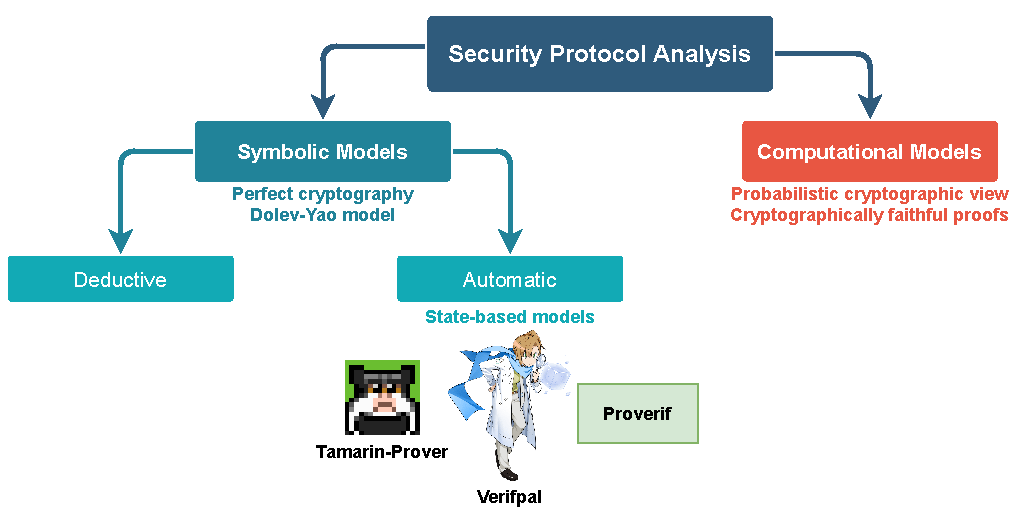
\includegraphics[scale=.9]{symbolic-computational-model}}
        \caption{Classification of tools}
        \label{fig:classification-of-tools}
    \end{figure}
}

These tools can be classified as shown in \cref{fig:classification-of-tools}. Two classes of tools can be identified. As the tools we are going to examine exploit the symbolic model, we will not explore the computational model (see \cite{ReconcilingComputationalSymbolic, SymbolicComputationalBlanchet, 10.1007/978-3-540-31987-0_12} for further readings). 

Let us briefly examine the symbolic model. This model assumes a Dolev-Yao \cite{Dolev-Yao} attacker. Moreover, cryptographic primitives are considered as black-box and are represented using function symbols, the messages are terms and the adversary can only use defined primitives. An important aspect to note of this model is that it assumes \textbf{perfect cryptography}. As an example, consider the case in which there are two function symbols (\textbf{enc} and \textbf{dec}, used to encrypt and decrypt), a message \textit{m} and a key \textit{k} and the following equality is defined:


\begin{equation}
\mbox{dec}\left(\mbox{enc}\left(m, k\right), k\right) = m
\end{equation}

Following from the equation $-$ and considering the perfect cryptography assumption $-$ it is possible to decrypt $\mbox{enc}\left(m, k\right)$ if and only if \textit{k} is known \cite{SymbolicComputationalBlanchet}.

We can further classify these tools in automatic and deductive. In particular, we will have a look at the internal reasoning and at some examples of three automatic tools: Tamarin-prover, Verifpal and Proverif.\clearpage
    % Section 2
% 2021-08-19
% Alessandro Zanatta

\section{Foundations}
\label{section:foundations}

In this section we are going to see a brief overview on the foundations of Tamarin-prover, Verifpal  and Proverif $-$ the three tools we are going to compare.


\subsection{Tamarin-prover}
Let us start with Tamarin\footnote{We will refer to Tamarin-prover as Tamarin for brevity.}. For a more
in-depth description and further information, see the Tamarin foundations paper \cite{TamarinFoundations} or the extended foundations paper \cite{TamarinFoundationsExtended}.

The security property model of Tamarin is based on labelled multiset rewriting rules to specify protocols and adversary capabilities, a guarded fragment\footnote{The guarded fragment used by Tamarin is basically a subset of formulas from the first order logic with additional constraints on the arguments. See \cite{FragmentFirstOrderLogicPaper} for a definition from a mathematical point of view.} of first order logic to specify security properties\footnote{These are known as \textit{lemmas} in Tamarin.} and functions and equational theories to model the algebraic properties of cryptographic protocols \cite{TamarinFoundations}.

Tamarin then applies a novel constraint-solving algorithm based on heuristics which tries to validate or falsify security properties.

\subsubsection{Multiset rewriting system}
The ingredients of Tamarin's multiset rewriting system are the following:

\begin{itemize}
    \item{Terms $-$ which can be thought of as messages;}
    \item{Facts $-$ which model information in the protocol and are composed by terms;}
    \item{State of the system $-$ which is represented using a \textit{multiset} of facts;}
    \item{Transition rules $-$ which defines the possible transitions from one state to another. We will use the following syntax: $\msr{L}{A}{R}$, where $L$, $A$ and $R$ are multisets of facts, respectively called premises, actions and conclusions;}
    \item{Trace $-$ a sequence $\left<A_1, \dots, A_n\right>$ of sets of ground facts (i.e. facts which do not contain any variable) denoting the sequence of \textit{actions} (or \textit{events}) that happened during the protocol execution.}
\end{itemize}

\subsubsection{Constraint-solving procedure}
\Cref{pseudocode:tamarin-solving-procedure} shows an high level view of the constraint-solving procedure of Tamarin. 

\begin{algorithm}
    \begin{algorithmic}
        \Function{Solve}{\textphi}
        \EndFunction
    \end{algorithmic}
    \caption{Tamarin's constraint solving procedure}
    \label{pseudocode:tamarin-solving-procedure}
\end{algorithm}

\subsection{Verifpal}
We will examine the analysis methodology

\subsection{Proverif}\clearpage
    % Section 3
% 2021-08-19
% Alessandro Zanatta

\section{Case study}
\label{section:case-study}

The full models of the following examples are freely available on github \cite{CaseStudies}.

\subsection{Diffie-Hellman key exchange}

We will examine three different models for the Diffie-Hellman key exchange protocol: anonymous, ephemeral and ephemeral with Perfect Forward Secrecy. This allows us to explore many advanced features and modelling techniques of each tool. \Cref{fig:dh-key-exchange} shows a schematic representation of the protocol.

In the anonymous version we model an un-authenticated Diffie-Hellman, where no security property can hold as the adversary is free to perform a man-in-the-middle attack \cite{MITM-DH}.

In the ephemeral version we model a client-server Diffie-Hellman exchange in which the server's half key is authenticated (e.g. by an X.509 certificate). The server is willing to execute the protocol with any client, but the server is always authenticated.

Finally, we model a Diffie-Hellman with post-compromise of ephemeral keys. This is how Perfect Forward Secrecy \cite{PFS} is usually tested in the symbolic model. Of course, secrecy of the exchanged messages will not hold.

\begin{figure}[t]
    \setmscoptions
    \begin{msc}{}
    \setmscscale{.7} 
    
    \declinst{client}{}{Client}
    \declinst{server}{}{Server}
    
    \action*{\parbox{3.5cm}{\centering
        Knows $g, p$\\
        $c \in \Z$\\
        $g_c := g ^ c \mod{p}$
    }}{client}

    \nextlevel[5]
    \mess{$g_c$}{client}{server}
    \nextlevel

    \action*{\parbox{3.5cm}{\centering
        Knows $g, p$\\
        $s \in \Z$\\
        $g_s := g ^ s \mod{p}$\\
        $K_{sc} := g_c ^ s \mod{p}$
    }}{server}

    \nextlevel[6]
    \mess{$g_s$}{server}{client}
    \nextlevel

    \action*{\parbox{3.5cm}{\centering
        $K_{cs} := g_s ^ c \mod{p}$
    }}{client}
    \nextlevel

    \end{msc}
    \centering
    \caption{Diffie-Hellman key exchange protocol}
    \label{fig:dh-key-exchange}
\end{figure}

\subsubsection{Implementation notes}

We will describe implementation details worth of note in the next paragraphs. Notice that we will use an incremental approach, describing only what was \textit{changed} between different versions. 

\paragraph{Anonymous} The implementation of the anonymous version is straightforward. We use two particular constructs for Proverif and Tamarin to store keys: tables and persistent facts, respectively. Both serve the same scope: store some permanent information (which is not, by default, available to the attacker). The first supports two operations: \textit{insert} and \textit{get}. The latter is, in essence, a \textit{fact} with the additional property of never being removed from the global state.

\paragraph{Ephemeral} In this version, the server half key needs to be authenticated\footnote{An additional requirement is that, while the half key cannot be mutated by the attacker, it must be available to it.}. In Verifpal there is a single (simple) way: guarded variables. Guarded variables (variables between square brackets) are not mutable by the attacker (but known by it). In Tamarin we model this with a simple private channel ruled by a passive attacker. This is done with the following multiset rewriting rule:


\lstset{language=tamarin}
\begin{lstlisting}
rule CertificateExchange:
    [ CertificateOut(x) ] --> [ CertificateIn(x), Out(x) ]
\end{lstlisting}

Finally, in Proverif we model this with a table, additionally making sure to output everything we insert into it. We could have also used a private channel, but that makes the verification of certain queries yield an inconclusive result.

\paragraph{Post-compromise} In tamarin, we define the following rule (for both client and server):

\lstset{language=tamarin}
\begin{lstlisting}
rule RevealClientEphemeralKey:
    [ ClientEphemeralKey(c) ]
  --[ RevealedClientEphemeralKey(c) ]->
    [ Out(c) ]
\end{lstlisting}

\begin{equation}
\msr{\fact{ClientEphemeralKey}{x}}{\fact{RevealedClientEphemeralKey}{x}}{\fact{Out}{x}}
\end{equation}

This actually models a \textit{generic} compromise rule. We can exploit timepoints in security properties to assert that the compromise must happen \textbf{after} some other event, making this a post-compromise.

In Proverif, we define a new process which simply outputs the ephemeral key in phase 1:

\lstset{language=proverif}
\begin{lstlisting}
let PostRevealClientEphemeralKey =
    phase 1;

    (* Get the client's ephemeral key and output it *)
    get ClientEphemeralKeyTable(c) in
    out(io, c);
    event PostRevealedClientEphemeralKeyTable(c);
    0.
\end{lstlisting}

\lstset{language=verifpal}
Modeling post-compromise in Verifpal requires using phases again. We can then use Verifpal's built-in construct for revealing terms: \lstinline{leaks x}.  
\begin{lstlisting}
phase [1]

principal Client [
    leaks c
]

principal Server [
    leaks s
]
\end{lstlisting}

\subsection{Needham-Schroeder public-key protocol}

\begin{figure}[t]
    \setmscoptions
    \begin{msc}{}
    \setmscscale{.7} 
    
    \declinst{alice}{}{Alice}
    \declinst{bob}{}{Bob}
    
    \action*{\parbox{3.5cm}{\centering
        Knows $K_{SA}, K_{PA}$\\
        Knows $K_{PB}$
    }}{alice}

    \action*{\parbox{3.5cm}{\centering
        Knows $K_{SB}, K_{PB}$\\
        Knows $K_{PA}$
    }}{bob}
    \nextlevel[4]

    \action*{\parbox{3.5cm}{\centering
        Generates $N_A$
    }}{alice}

    \nextlevel[3]    
    \mess{$\left\{N_A, A\right\}_{K_{PB}}$}{alice}{bob}
    \nextlevel


    \action*{\parbox{3.5cm}{\centering
        Generates $N_B$
    }}{bob}

    \nextlevel[3]
    \mess{$\left\{N_A, N_B\right\}_{K_{PA}}$}{bob}{alice}
    \nextlevel[2]
    \mess{$\left\{N_B\right\}_{K_{PB}}$}{alice}{bob}

    \end{msc}

    \centering
    \caption{Simplified Needham-Schroeder Public-key protocol}
    \label{fig:NSPK}
\end{figure}

The next case-study is the Needham-Schroeder Public-key protocol. Two versions are considered: the flawed version and the fixed one (by Lowe \cite{NSPK_LoweGavin}). A schematic representation of the protocol is shown in \cref{fig:NSPK}, which assumes that clients already know each others public keys.

\subsubsection{Implementation notes}

In order to re-discover the attack, we model the protocol in a way that allows the attacker to decide whom the honest initiator executes the protocol with. The responder, however, only engages with the honest initiator.

\paragraph{Flawed} \clearpage
    % Section 4
% 2021-08-19
% Alessandro Zanatta

\section{Features comparison}
\label{section:features-comparison}

\comment{
Tamarin
    Pros:
        - More expressive formulas for security properties
        - Sound and complete
        - Can prove observational equivalence
        - Possibility of manually guiding the proof when heuristics fail to do so automagically
        - Can model many algebraic properties of groups for DH key exchanges (comes with higher computational cost!)
        - Can model xor and elliptic curve operations
        - Supports user defined equational theories
        - More flexibility on post compromise properties using timepoints, but lemmas become more verbose
    Cons:
        - Probably harder to model
        - Slower (do benchmarks!!)


Proverif
    Pros:
        - Long history
        - Can prove observational equivalence
        - Supports user defined equational theories
    Cons:
        - Uses an old-style syntax
        - CANNOT model many algebraic properties of groups for DH key exchanges (only commutativity)


Verifpal
    Pros:
        - Very simple to use (both model specification and queries), while being expressive enough for most use cases
        - Possibility to translate to proverif/coq (even though its limited)
        - Very intuitive language
    Cons:
        - There may be queries that CANNOT be expressed (try finding a counterexample!)
        - CANNOT prove observational equivalence
        - It's very recent, still in beta
        - CANNOT model many algebraic properties of groups for DH key exchanges (only commutativity ???)
        - does NOT support user-defined equational theories
        - Does NOT allow to express injectivity
        - Does NOT produce a graphical representation of traces automatically

}\clearpage
    % Section 1
% 2021-08-19
% Alessandro Zanatta

\section{Conclusions}
\label{section:conclusions}

Conclusions here\clearpage
    
    % Bibliography
    \bibliography{references}
 % Print all bibliography references

\end{document}